% Schematic representation of corona poling
% From NLO of organic molecules and polymers, Singh/Miyata.
% Author: Orlando Torres (2016)
\documentclass{standalone}
\usepackage{amsmath} % Required for \varPsi below
\usepackage{tikz,pgfplots}
\usetikzlibrary{shapes.geometric}
\usetikzlibrary{circuits}
\usetikzlibrary{circuits.logic.US}
\usetikzlibrary{circuits.logic.IEC}
\begin{document}
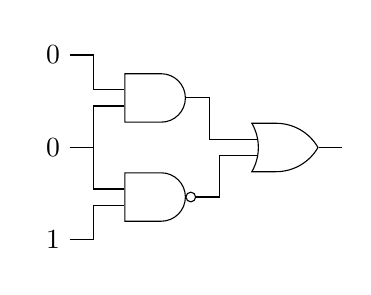
\begin{tikzpicture}[circuit logic US]
\matrix[column sep=7mm]
{
\node (i0) {0}; & & \\
& \node [and gate] (a1) {}; & \\
\node (i1) {0}; & & \node [or gate] (o) {};\\
& \node [nand gate] (a2) {}; & \\
\node (i2) {1}; & & \\
};
\draw (i0.east) -- ++(right:3mm) |- (a1.input 1);
\draw (i1.east) -- ++(right:3mm) |- (a1.input 2);
\draw (i1.east) -- ++(right:3mm) |- (a2.input 1);
\draw (i2.east) -- ++(right:3mm) |- (a2.input 2);
\draw (a1.output) -- ++(right:3mm) |- (o.input 1);
\draw (a2.output) -- ++(right:3mm) |- (o.input 2);
\draw (o.output) -- ++(right:3mm);
\end{tikzpicture}
\end{document}